\documentclass[letterpaper]{article}
\usepackage[spanish]{babel}
\usepackage{fixltx2e}
\usepackage{graphicx}
\usepackage[utf8]{inputenc}
\usepackage{hyperref}
\usepackage{mathtools}
\usepackage{numprint}

\npthousandsep{\thinspace}
\npthousandthpartsep{}
\npdecimalsign{,}

\begin{document}

\title{Evaluación del informe\\"Generación de códigos únicos para unidades geográficas"}
\author{Sylvain Lesage\\
  \texttt{slesage@adsib.gob.bo}}
\date{\today}
\maketitle
 
\begin{abstract}
Abstract...
\end{abstract}

\section{Antecedentes}

\section{Características de la propuesta INE}

Coordenadas en la proyección cónica conforme de Lambert \cite[p.~33]{sunit07}. Ver el cuadro \ref{tab:lambert}.

\begin{table}
	\centering
	\begin{tabular}{|l|l|}
		\hline
		Falso origen & lat: 24º S, lon: 64º \\
		Meridiano central & 64º00' Oeste \\
		Latitud de origen & 24º00' Sur \\
		1ro Paralelo estándar & 11º30' Sur \\
		2do Paralelo estándar & 21º30' Sur \\
		Falso Este & 1.000.000m \\
		Falso Norte & 0m \\
		\hline	
	\end{tabular}
	\caption{Parámetros de la proyección cónica conforme de Lambert para Bolivia}
	\label{tab:lambert}
\end{table}

Cada polígono (manzano, comunidad) esta resumido a un solo punto: su centroide. Se lo calcula con Quantum GIS versión Dufour.

Cálculos - ver programa ... (gitlab)

\subsection{Definición del código}

Dados \(x\) y \(y\) las coordenadas de un punto en la proyección cónica conforme de Lambert, el código único \(z\) esta definido por:

\[z = \lfloor r \exp{\theta} \rfloor\]

donde

\[r = \sqrt{x^2+y^2} \]

y

\[\theta = \arctan{\frac{y}{x}} + \pi \]

Nota: el documento base omite la adición de \(\pi\) en el cálculo de \(\theta\).

\subsection{Número de códigos}

A partir del archivo de los límites de Bolivia \cite{datos:limites_bolivia}, podemos calcular los valores límites de las coordenadas \(x\) y \(y\) de todos los puntos del territorio en la proyección cónica conforme de Lambert. La coordenada \(x\) se encuentra en el intervalo \([\numprint{391248}\,\mathrm{m}, \numprint{1689926}\,\mathrm{m}]\) y la coordenada \(y\) en el intervalo \([\numprint{119437}\,\mathrm{m}, \numprint{1583581}\,\mathrm{m}]\).

Podemos deducir el valor límite de las variables polares \(r\) y \(\theta\). Tomar en cuenta que son valores límites, correspondiendo a las esquinas del \emph{bounding box} (cuadrado delimitado por \(x_{min}\), \(x_{max}\), \(y_{min}\) y \(y_{max}\)) de Bolivia: no necesariamente existe un punto con estos valores de \(r\) y \(\theta\). El radio \(r\) se encuentra en el intervalo \([\numprint{614506}\,\mathrm{m}, \numprint{1814299}\,\mathrm{m}]\) y el ángulo \(\theta\) en el intervalo \([\numprint{3.27}\,\mathrm{rad}, \numprint{4.44}\,\mathrm{rad}]\).

Según la formula de cálculo del código \(z\), esté crece con \(r\) y \(\theta\), por lo cual podemos calcular los valores límites del código \(z\) (con la misma advertencia: no necesariamente existe un punto en Bolivia que tenga estos valores extremos del código). Las estimaciones mínima y máxima del código \(z\) son respectivamente \(\numprint{17493127}\) y \(\numprint{126692164}\). Por ende, podemos concluir que existe, en el territorio Boliviano, como estimación superior, \(\numprint{109199037}\) códigos diferentes.

El cuadro \ref{tab:variables} presenta un resumen de todos los valores.

\begin{table}
	\centering
	\begin{tabular}{|l|l|}
		\hline
		Variable & Valores \\
		\hline
		\(x\) & entre \(\numprint{391248}\,\mathrm{m}\) y \(\numprint{1689926}\,\mathrm{m}\) \\
		\(y\) & entre \(\numprint{119437}\,\mathrm{m}\) y \(\numprint{1583581}\,\mathrm{m}\) \\
		\hline
		\(r\) & entre \(\numprint{614506}\,\mathrm{m}\) y \(\numprint{1814299}\,\mathrm{m}\) \\
		\(\theta\) & entre \(3.27\,\mathrm{rad}\) y \(4.44\,\mathrm{rad}\) \\
		\hline
		código \(z\) & entre \(\numprint{17493127}\) y \(\numprint{126692164}\) \\
		número de códigos & menos de \(\numprint{109199037}\) códigos diferentes \\
		\hline
	\end{tabular}
	\caption{Características del código \(z\)}
	\label{tab:variables}
\end{table}

\subsection{Precisión espacial del código}

Tomando en cuenta que la superficie del territorio de Bolivia\footnote{según http://es.wikipedia.org/wiki/Bolivia} es aproximadamente de \(\numprint{1098581}\,\mathrm{km^{2}}\), podemos calcular que la superficie promedio del territorio correspondiendo a cada valor del código es de \(\numprint{10060}\,\mathrm{m^{2}}\), lo que equivale un cuadrado de \(100\,\mathrm{m}\) de lado. Significa que para valor del código \(z\), existe una hectárea del territorio nacional donde todos los puntos comparten el mismo valor de \(z\), o sea donde el código \(z\) no permite discriminar entre los puntos incluidos. Podemos expresar este valor como el nivel de precisión del código.

Podemos también calcular la forma de las áreas \emph{equi-código}. Los límites de estas áreas son definidos, para un valor específico de \(z\), y para los ángulos \(\theta\) correspondiendo a Bolivia, por los valores siguientes:

\[
\left\{
\begin{array}{l l}
r_{min} = z \exp{-\theta} \\
r_{max} = (z+1) \exp{-\theta}
\end{array} \right.
\]

Calculamos la geometría de las nueve áreas correspondiendo al código de cada capital departamental de Bolivia. La figura \ref{fig:areas_por_capital} representa estas áreas. Aparece claramente que les áreas \emph{equi-código} forman \emph{franjas} muy estrechas que cruzan toda Bolivia. Por ejemplo, el área que contiene el punto central de La Paz mide \(\numprint{1224}\,\mathrm{km}\) de largo y solamente \(\numprint{2.24}\,\mathrm{cm}\) de ancho en promedio (con un ancho mínimo de \(\numprint{1.18}\,\mathrm{cm}\) y un ancho máximo de \(\numprint{3.80}\,\mathrm{cm}\)). Su superficie es de \(\numprint{19292}\,\mathrm{m^{2}}\), lo que equivale a un cuadrado de \(\numprint{138}\,\mathrm{m}\) de lado.

El detalle de estas medidas para las nueve capitales de Bolivia se encuentra en el cuadro \ref{tab:capitales}. La figura \ref{fig:areas_por_capital} y su acercamiento en la ciudad de Santa Cruz (figura \ref{fig:areas_por_capital_santacruz_cochabamba}) muestran que por casualidad, las áreas \emph{equi-código} de Santa Cruz y Cochambamba son casi superpuestas, lo que significa que posiblemente varios manzanos de Santa Cruz y de Cochabamba compartan el mismo código.

\begin{table}
	\centering
	\begin{tabular}{|l|l|}
		\hline
		Variable & Valores \\
		\hline
		superficie de Bolivia & \(\numprint{1098581}\,\mathrm{km^{2}}\) \\
		precisión del código & \(\numprint{10060}\,\mathrm{m^{2}}\), o sea una hectárea, como promedio\\
		\hline
	\end{tabular}
	\caption{Precisión espacial del código \(z\)}
	\label{tab:variables}
\end{table}

\begin{figure}[p]
    \centering
    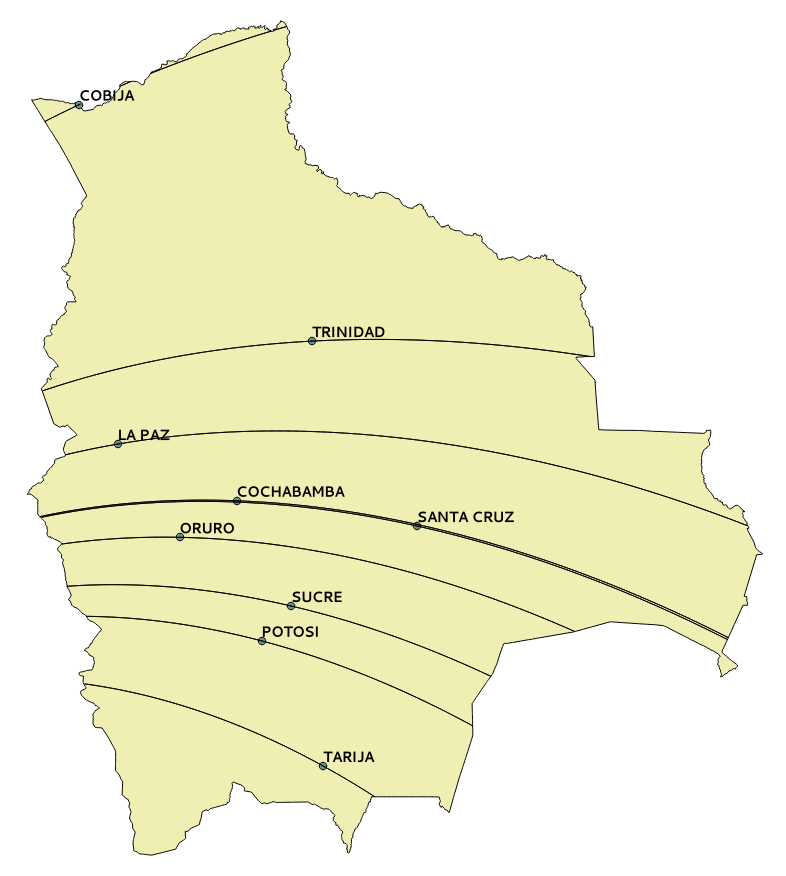
\includegraphics[width=0.8\textwidth]{resultados/area_equi_codigo_9_capitales.png}
    \caption{Área \emph{equi-código} para cada capital departamental de Bolivia. Nota: las áreas parecen líneas porque son extremadamente estrechas (\(\numprint{2.24}\,\mathrm{cm}\) en promedio)}
    \label{fig:areas_por_capital}
\end{figure}

\begin{figure}[p]
    \centering
    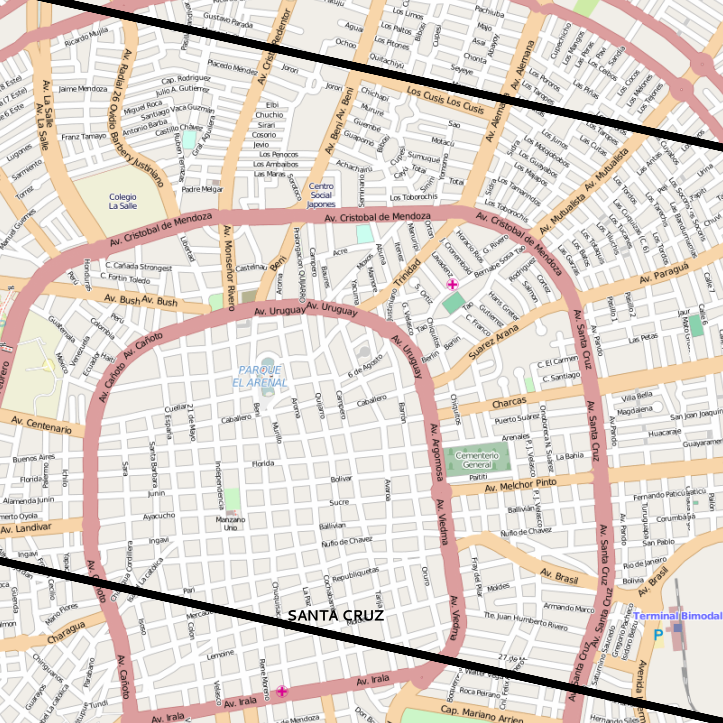
\includegraphics[width=0.8\textwidth]{resultados/area_equi_codigo_santacruz_cochabamba.png}
    \caption{Acercamiento sobre la ciudad de Santa Cruz para las áreas \emph{equi-código} para Santa Cruz y Cochabamba. Toda una franja de la ciudad de Santa Cruz (banda negra arriba) comparte el mismo código que la ciudad de Cochambamba}
    \label{fig:areas_por_capital_santacruz_cochabamba}
\end{figure}

\begin{table}
	\centering
	\begin{tabular}{|l|l|l|l|l|}
		\hline
		Capital & Superficie & Eq. lado de cuadrado & Largo & Ancho (promedio) \\
		\hline
		Cobija & \(\numprint{3377}\,\mathrm{m^{2}}\) & \(\numprint{58}\,\mathrm{m}\) & \(\numprint{352}\,\mathrm{km}\) & \(\numprint{2.24}\,\mathrm{cm}\) \\
		Trinidad & \(\numprint{12957}\,\mathrm{m^{2}}\) & \(\numprint{113}\,\mathrm{m}\) & \(\numprint{983}\,\mathrm{km}\) & \(\numprint{2.24}\,\mathrm{cm}\) \\
		La Paz & \(\numprint{19292}\,\mathrm{m^{2}}\) & \(\numprint{113}\,\mathrm{m}\) & \(\numprint{1224}\,\mathrm{km}\) & \(\numprint{2.24}\,\mathrm{cm}\) \\
		Cochabamba & \(\numprint{21072}\,\mathrm{m^{2}}\) & \(\numprint{145}\,\mathrm{m}\) & \(\numprint{1244}\,\mathrm{km}\) & \(\numprint{2.24}\,\mathrm{cm}\) \\
		Oruro & \(\numprint{15302}\,\mathrm{m^{2}}\) & \(\numprint{145}\,\mathrm{m}\) & \(\numprint{919}\,\mathrm{km}\) & \(\numprint{2.24}\,\mathrm{cm}\) \\
		Sucre & \(\numprint{13106}\,\mathrm{m^{2}}\) & \(\numprint{114}\,\mathrm{m}\) & \(\numprint{760}\,\mathrm{km}\) & \(\numprint{2.24}\,\mathrm{cm}\) \\
		Potosí & \(\numprint{12907}\,\mathrm{m^{2}}\) & \(\numprint{113}\,\mathrm{m}\) & \(\numprint{701}\,\mathrm{km}\) & \(\numprint{2.24}\,\mathrm{cm}\) \\
		Tarija & \(\numprint{10864}\,\mathrm{m^{2}}\) & \(\numprint{104}\,\mathrm{m}\) & \(\numprint{540}\,\mathrm{km}\) & \(\numprint{2.24}\,\mathrm{cm}\) \\
		Santa Cruz & \(\numprint{21064}\,\mathrm{m^{2}}\) & \(\numprint{145}\,\mathrm{m}\) & \(\numprint{1241}\,\mathrm{km}\) & \(\numprint{2.24}\,\mathrm{cm}\) \\
		\hline
	\end{tabular}
	\caption{Área \emph{equi-código} para cada capital departamental de Bolivia}
	\label{tab:capitales}
\end{table}

\section{Alternativas}

\section{Tabla comparativa entre los códigos}

\section{Conclusión y recomendaciones}

\begin{thebibliography}{99}

\bibitem{sunit07}
  Sistema Unico de Información de la Tierra,
  \emph{Normas técnicas para la administración de la información georeferenciada a nivel nacional}.
  Resolución Ministerial Nº~338 del MDRAyMA,
  2007.

\bibitem{datos:limites_bolivia}
  Límite Nacional de Bolivia,
  Formato Shapefile,
  GADM,
  \url{http://www.gadm.org},
  \url{http://biogeo.ucdavis.edu/data/gadm2/shp/BOL_adm.zip}

\end{thebibliography}

\end{document}
